\newpage
\section{Introduction to injections}
\genHeader

This short introduction will show you how to implement small methods by adding handwritten code to classes generated from your model. Injections are inspired by
partial classes in C\#, and are our preferred way of providing a clean separation between generated and handwritten code. 

Let's implement the \texttt{removeCard} method, declared in the \texttt{Partition} EClass. In order to `remove' a card from a partition, all one needs to do is
disable the link between them. Don't forget that (according to the signature) not only does \texttt{removeCard} have to pass in a \texttt{Card}, it must return
one as well.

\begin{itemize}

\item[$\blacktriangleright$] From your working set, open ``gen/LearningBoxLanguage.impl/Part\-it\-ionImpl.java'' and enter the following code in the
\texttt{removeCard} declaration, starting at approximately line 358. Do not remove the first comment, which is necessary to indicate that this code is written
by the user and needs to be extracted automatically as an injection. Please also do not copy and paste the following code -- the copying process will most
likely add invisible characters that eMoflon is unable to handle.

\vspace{0.5cm}

\begin{figure}[htbp]
        \centering
        \begin{lstlisting}[language=Java, keywordstyle={\bfseries\color{purple}}, backgroundcolor=\color{white}]
    public Card removeCard(Card card) {
        // [user code injected with eMoflon]
        if (card != null){
        	card.setCardContainer(null);
        }
        return card;
    }
        \end{lstlisting}
        \caption{Implementation of \texttt{removeCard}}
        \label{code:addToStringRep_impl}
\end{figure}

\vspace{0.5cm}

\item[$\blacktriangleright$] Save the file, then right-click either on the file in the package explorer, or in the editor window, and choose ``eMoflon/
Create/Update Injection for class'' from the context menu (Fig.~\ref{eclipse:injection_create_injection}).

\begin{figure}[htbp]
    \centering
    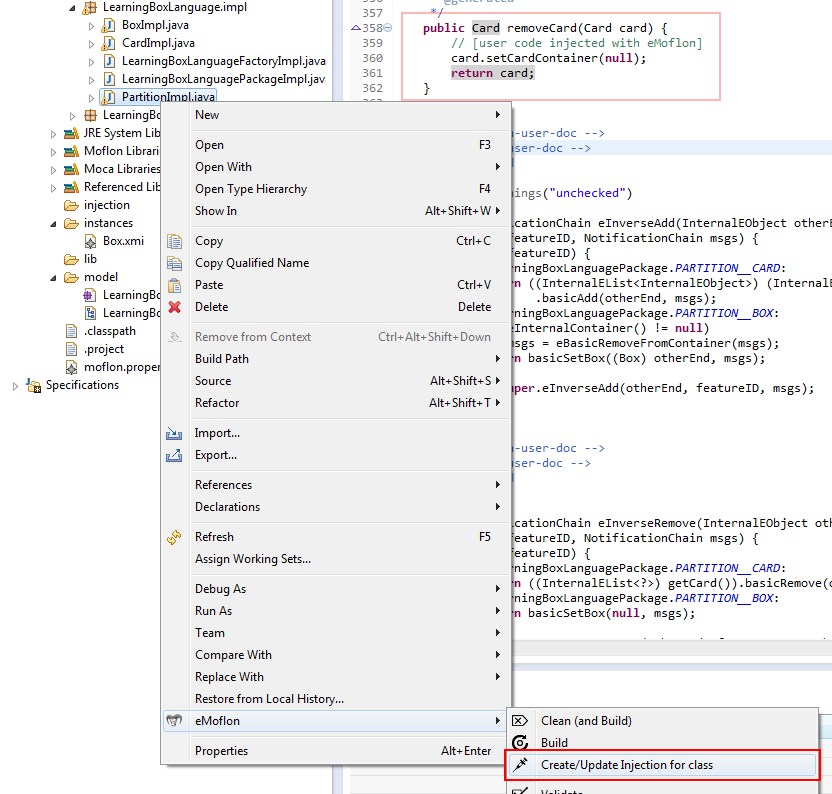
\includegraphics[width=\textwidth]{eclipse_createInjection}
    \caption{Create a new injection}
    \label{eclipse:injection_create_injection}
\end{figure}

\item[$\blacktriangleright$] This will create a new file in the ``injection'' folder of your project with the same package and name stucture as the Java class,
but with a new \texttt{.inject} extension (Fig.~\ref{eclipse:injection_folder}).

\begin{figure}[htbp]
    \centering
    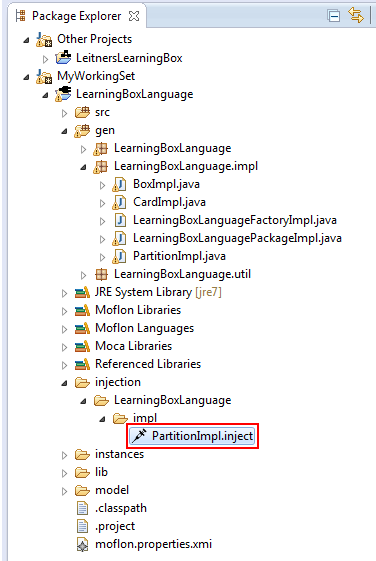
\includegraphics[width=0.5\textwidth]{eclipse_injectionFolder}
    \caption{Partition injection file}
    \label{eclipse:injection_folder}
\end{figure}

\item[$\blacktriangleright$] Double click to open and view this file. It contains the definition of a \textit{partial class}
(Fig.~\ref{eclipse:injection_partialClassPartition}).

\begin{figure}[htbp]
    \centering
    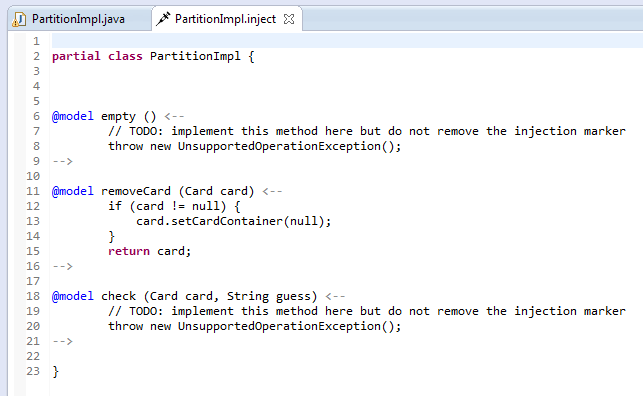
\includegraphics[width=0.9\textwidth]{eclipse_partialClassPartition}
    \caption{Generated injection file for \texttt{PartitionImpl.java}}
    \label{eclipse:injection_partialClassPartition}
\end{figure}

\clearpage

\item[$\blacktriangleright$] As a final step, clean and build your metamodel to check that the code is generated and injected properly.

\item[$\blacktriangleright$] That's it! While injecting handwritten code is a remarkably simple process, it is pretty boring and low level to call all those
setters and getters yourself. We'll return to injections for establishing two simple methods in Part III using this strategy, but we'll also learn how to
implement more complex methods using Story Diagrams.
 
\end{itemize}
